\chapter{Introduction}


The human body has always been an inspiration for many technologies. Scientists have successfully achieved to understand the mechanics behind different parts of the human body and have created models that imitate the functionalities of the studied parts. The human brain is one of the most complex organs in the human body \citep{nolte2002human}, and we do still not fully understand its inner workings. Creating machines that can achieve human capabilities such as high-level cognition associated with conscious perception is a human dream since a long time. However, before such a goal can even remotely be achieved, we need to understand how information is processed in the brain, how that would be replicated by machines, and how models of it can be created that target specific functions of the brain and replicate their behavior in connection with other parts of the body.

Due to technical and ethical reasons, neuroscientist may not be able to directly investigate certain parts of the brain and experiment on their responses. Therefore, to avoid experimenting in vivo and at the same time attaining realistic results, an embodied simulation framework like presented in \citet{10.3389/fninf.2022.884180} might be used to simulate the brain at scale in order to capture the contributions of multiple brain regions involved in purposeful actions.

Successfully understanding the processes in the brain that create phenomena such as creativity, dreaming and consciousness crucially depends on efficient and easy to use \emph{neural simulators}, the development of which strongly depends on the interaction between researches from both the fields of computer science and neuroscience. Such interactions may lead to better quality and feature-richness of the simulation frameworks and as a result to a better understanding of the human mind. One building block in the neural simulation landscape are tools for the creation of neuron and synapse models, which are the basic processing elements of the brain. 


\section{The structural and functional unit of the neural system}

The nervous system consists mainly of two types of cells: \emph{neuron} and \emph{glia}. The neurons are information messengers that use electrical impulses and chemical signals to transmit information between different areas of the brain and between the brain and the rest of the nervous system. Everything we \emph{think}, \emph{feel} and \emph{do} would be impossible without the work of neurons. Glial cells provide support for neurons in the form of nutrients and other chemicals and play an important role in keeping the chemical environment of the brain in a good working condition, for example by taking up left-over neurotransmitters or surplus ions.

\begin{figure}[ht!]
  \centering
  \includegraphics[width=\linewidth]{src/pic/neuron.eps}
  \caption{\textbf{The neuron \cite[taken from][]{introductiontopsychology}}. Neurons consist of three major components: The \emph{cell body} (also known as the \emph{soma}) is the core of the neuron containing the nucleus of the cell. The \emph{dendrites} are a tree-like, branched structure collecting information from other cells and sending it to the soma. The \emph{axon} is a long segmented protrusion transmitting information away from the cell body towards other connected neurons. Moreover, the axon is surrounded by a layer of fatty tissue known as the \emph{myelin sheath}. It acts as an insulator and allows faster transmission of the electrical signal by preventing the electrical charge from shorting out.}
  \label{fig:neuron}
\end{figure}

\begin{figure}[ht!]
  \centering
  \includegraphics[width=\linewidth]{src/pic/synaptic.eps}
  \caption{\textbf{The synapse \citep[taken from][]{Neurotransmitters}}. Most communication between neurons occurs at specialized structures called \emph{synapses}. The synapse is the area where two neurons come close enough that they are able to pass a chemical signal (\emph{neurotransmitters}) from one to another. The gap between the neurons where this chemical exchange takes place is called the synaptic cleft. Neurotransmitters are packaged into small sacs called vesicles (blue circles in the figure). Each vesicle can contain thousands of neurotransmitter molecules. When the pre-synaptic neuron gets active, this causes the vesicles to fuse with the pre-synaptic membrane and release the neurotransmitter molecules into the cleft. Once the neurotransmitter are in the synaptic cleft, they interact with the receptors on the post-synaptic membrane, bind with them, and may cause an action to occur in the post-synaptic cell.}
  \label{fig:synapse}
\end{figure}

The whole process of communication between neurons as depicted in \autoref{fig:neuron} is based on passing an \emph{electrochemical} signal from one neuron (called the \emph{pre-synaptic} neuron) to many neurons (called \emph{post-synaptic} neurons). A received electrical impulse travels through the neuron and a chemical reaction is triggered to transmit the signal to the next neuron. When a signal is received at the level of the \emph{dendrites}, it is transmitted to the \emph{soma} in the form of an electrical signal. If the accumulated signal is strong enough, it may be forwarded to the axon and afterwards to the synapses. Reaching these terminal stations, a chemical reaction takes place, emitting \emph{neurotransmitters}, which are transported to connected neurons across the space between the cells. See \autoref{fig:synapse} for details.

We distinguish three states (or phases) that a neuron can undergo, the \emph{resting state}, the \emph{action potential} and the \emph{hyper-polarization} as depicted in \autoref{fig:action_potential}. In the \emph{resting state}, the interior of the cell contains a greater number of negatively charged ions than the outside of the cell. This imbalance leads to a measurable \emph{membrane potential} of about -55 mV. If the first segment of the axon is stimulated by an incoming signal traveling down from the \emph{dendrites} and if the impulse is strong enough to reach a certain \emph{threshold}, the segment opens its voltage-gated ion-channels, allowing positively charged sodium ions ($Na^{+}$) to enter. This change in electrical charge is known as an \emph{action potential} or \emph{spike} due to the form of the excursion of the membrane potential. Once an action potential is elicited, the number of positively charged ions exceeds the number of negative ions in the segment, and it becomes temporarily positively charged. As a consequence, a similar electrical change occurs in the next segment, allowing the electrical impulse to travel along the axon as a wave until it reaches the synapses. It is important to note here that when the signal passes the next segment, the prior segment's gates close again and the potential returns to its original state.


\begin{figure}[ht!]
  \centering
  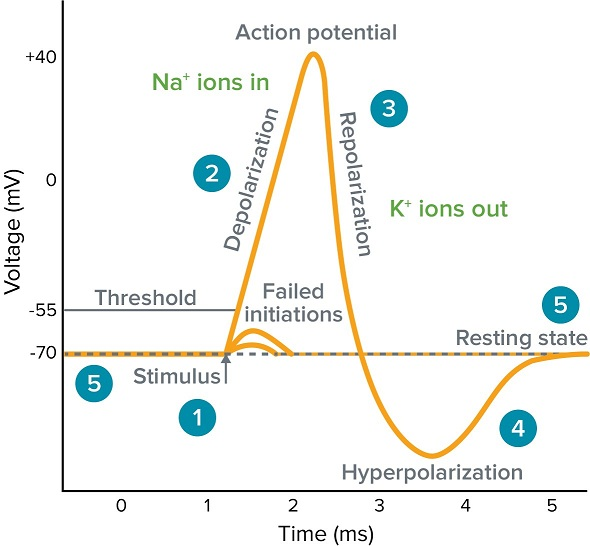
\includegraphics[width=\linewidth]{src/pic/what-is-action-potential.jpg}
  \caption{\textbf{The Action potential \citep[taken from][]{what-action-potential}}: (1): Stimulus triggers the rapid change in voltage or action potential. A sufficient current must be accumulated in the cell in order to raise the voltage above the threshold voltage to start membrane depolarization. (2): Depolarization is depicted as the rising phase, and it occurs when the sodium channels in the cellular membrane open causing a large influx of sodium ions. (3): Membrane Repolarization results from rapid sodium channel inactivation as well as a large efflux of potassium ions resulting from activated potassium channels. (4): Hyperpolarization is a lowered membrane potential caused by the efflux of potassium ions and closing of the potassium channels. (5): Resting state is when membrane potential returns to its resting voltage before being stimulated.}
  \label{fig:action_potential}
\end{figure}

An important property of the action potential is that it cannot be partial. It is that the neuron either \emph{fires} completely, such that the action potential travels all the way down the axon, or it does not fire at all. After firing a spike, the neuron is not able to instantly fire again due to the depletion of its neurotransmitter vesicles. This is true even if other electrical impulses are being accumulated at the dendrites. This period of \emph{hyper-polarization} is also called the \emph{refractory period} of the neuron.

When an axonal action potential reaches the terminal stations, the electrical impulse signals them to release neurotransmitters into the synapse. These neurotransmitters travel across the synaptic space between the terminal stations of one neuron and the dendrites of the others, where they bind to specific receptors on the dendrites of the post-synaptic neuron. Neurons may have the property of either having an \emph{excitatory} or \emph{inhibitory} effect to their post-synaptic neurons. Neurotransmitters exhibiting an excitatory increase the neuron's likelihood to fire, while inhibitory neurotransmitters decrease the cell's likelihood to fire. Given that different neurotransmitters arrive at the dendrites, the neuron will be influenced by both excitatory and inhibitory signals. The neuron accumulates both types of signals and when the total effect of the excitatory signals are greater than the total effect of the inhibitory signals, the neuron moves closer to its signal transduction threshold. Reaching the threshold, the signal is transmitted via the dendrite and the process begins anew in the next cell.

Gaining new knowledge, the connection between neurons strengthen. This is called long-term potentiation (\emph{LTP}) and it is an example of synaptic plasticity. It underlies the process of learning and memory retention. New memories are formed when neurons establish new connections, or strengthen the existing synapses.

\section{Neuronal simulation}

A cubic millimeter of mouse cortex contains about $9×10^4$ neurons, $7×10^8$ synapses \citep{faisal2005ion}. This tremendous number of neurons and connections makes it hard to conquer the overall complexity of the brain. Computer simulations can be a helping tool, but they have to be very efficient  in simulating the targeted parts and representing the available resources.

A neural simulator is a piece of software that would allow the user to specify models at a high level language by specifying the behavior of the models in a standard mathematical notation. The simulators should implement a computationally efficient algorithms and support a large-scale modelling and complex biophysical models. In order to minimize the learning and development time, the simulators should come with an extra component that transforms the user written model in the high level language into a low level language such as C++. An advantage of such component is that the user won't require an expertise in programming nor the knowledge of neural simulation algorithm. Additionally, the generated low level code can be targeted to any chosen hardware configuration without the need of adjusting the original code that was written in the high level language and thus the model can be at the same time optimized for CPU as well for running optimally in a specific GPU environment. Both, the neural simulator NEST \citep{gewaltig2007nest} and Brian \citep{10.3389/neuro.11.005.2008} handles the connectivity of the neuron in the brain as a Graph $G$ \citep{bondy1976graph} with the neurons being the set of nodes building the ensemble $ \mathcal{V}$ and the synapse as the connections between the nodes building the ensemble $ \mathcal{E}$. Each of the neurons and synapses in both simulators may have different properties that replicate their biological properties, and they can be set before running the simulation.

The \emph{neural simulation tool NEST} \citep{gewaltig2007nest, spreizer_sebastian_2022_6368024} is capable of simulating large neuronal networks with different neuron and synapse models. NEST is written in C++ and employs OpenMP for in-node parallelization using threads and the message passing-interface MPI \citep{clarke1994mpi} for distributed simulations. Its Python interface \citep[\emph{PyNEST};][]{10.3389/neuro.11.012.2008} makes it easy for users to run the simulations. Neuron models may be anything from simple \emph{point neurons} like the \emph{integrate-and-fire} neuron to complex compartmental neurons. While synapses may either be \emph{static} or have a variant weight that changes over time according to a \emph{plasticity} algorithm. NEST supports a variety of algorithms for synaptic plasticity. Examples for such algorithms are spike-timing-dependent plasticity (STDP), short-term plasticity (STP), or third-factor neuromodulated weight dynamics.

The neural network in NEST is generated from neurons and their connections using high-level API functions in PyNEST. The most essential functions are \texttt{Create()}, which is responsible for creating instances of the desired neuron models, \texttt{Connect()}, which connects the neurons and shapes the topology of the neural network, and \emph{Simulate()}, which drives the state of the dynamic system in time. The type of the synapse model used between the pre-synaptic neuron and the post-synaptic neuron is defined in the \texttt{Connect()} function. \autoref{lst:simple_simulation} shows a simple example of how to create two neurons and connect them using a specific synapse type and run the simulation.\\

\begin{figure}[ht!]
  \centering
\begin{lstlisting}[language=Python, label=lst:simple_simulation, caption={Every simulation script using PyNEST starts with importing the \texttt{nest} module in Python. In line 4, we create two Hodgkin-Huxley neurons as instances of the \emph{hh\_psc\_alpha\_gap} model. In line 5, we set a background current of 100.0 pA for both neurons. Line 6 modifies the initial membrane potentials of the first neuron instance to be at -10.0 mV. In line 8, we create a \texttt{voltmeter} to record the membrane potential of both neurons. In line 11, we connect the first neuron with the second neuron, and vice-versa using the \emph{gap\_junction} synapse model. Finally, we connect the voltmeter to the neurons to record their membrane potential over the course of the simulation in line 15 and run the simulation for 10.0 milliseconds in the last line by calling the \texttt{Simulate()} function.}, captionpos=b]
import nest

# Create neurons and devices
neurons = nest.Create('hh_psc_alpha_gap', 2)
neurons.I_e = 100.0
neurons[0].V_m = -10.0

vm = nest.Create('voltmeter', params={'interval': 0.1})

# Connect neurons and devices
nest.Connect(neurons, neurons,
    {'rule': 'all_to_all', 'allow_autapses': False},
    {'synapse_model': 'gap_junction', 'weight': 0.5})

nest.Connect(vm, neurons, 'all_to_all')

# Simulate the neural network
nest.Simulate(10.0)
\end{lstlisting}
  %\caption{The Simulation script imports without \emph{JIT}}
  %\label{fig:imports_without_jit}
\end{figure}

Being a research tool, NEST is constantly applied to new use cases and the set of built-in neuron and synapse models is by definition never complete. In order to not restrict users to only the models that come with NEST, they can create custom neuron and synapse models with the NEST Modelling Language \emph{NESTML} \citep{plotnikov2016nestml, linssen_charl_a_p_2022_5784175}. NESTML allows users to express models by specifying their state variables, parameters, equations, and optionally a procedural description of how the state is to be updated during the simulation. Such models can then be used in simulation studies by loading the generated and complied model libraries at runtime into NEST. NESTML itself is written in Python and consists of two parts: The first is a language specification that is heavily based on the syntax of Python, but also provides domain concepts like physical units and differential equation as first class concepts. Each custom model in NESTML is defined by its name in the \emph{neuron} block of the language and the specified name is used for generating the library code in C++ and for using the model in the simulation script. The second part of NESTML is a tool chain that takes a model description and produces C++ code and the boilerplate code required to compile the model into a dynamically loadable library. The most important function in the Python interface to NESTML (\emph{PyNESTML}) is the function \texttt{generate\_nest\_target()}, which generates an extension module for NEST given one or more \texttt{.nestml} files. After installing the library, instances of the model can be created using PyNEST's \texttt{Create()} function and connected with other elements in the network using the \texttt{Connect()} function.

\begin{figure}[ht!]
\centering
\begin{lstlisting}[language=Python, label=lst:nestml_without_synapse, caption={Generating extension module code: The \texttt{generate\_nest\_target} function generates code only for a neuron model. The minimum required parameter of the function is the \texttt{input\_path} that points to the location of the model. Once the code is generated, the built libraries can be loaded into NEST using the \texttt{Install} function by providing the name of the module (\emph{simple\_module}). Once the model is installed in NEST, we can create instances of the model by calling the \texttt{Create()} function with the model name being the name that was written in the NESTML file in the neuron block.}, captionpos=b]
# Generate code only for a neuron model
generate_nest_target(
    input_path="neuron_model.nestml",
    target_path="where_to_generate_the_code",
    module_name="simple_module",
    logging_level="ERROR")

# Install the extension module
nest.Install("simple_module")

# Create instances of the model
neuron = nest.Create("neuron_model", 2)

# Create a simple network
nest.Connect(neurons[0], neurons[1],
    syn_spec={'synapse_model': "any_built_in_synapse_type"})
\end{lstlisting}
\end{figure}

If there are no interdependent variables between a neuron and synapse model, as in the case of neurons connected via static synapses or dynamic synapses that only depend on the spikes that are transmitted via them and not on any other factors, the code for the neuron can be generated without specifying the synapse model. An example for the NESTML invocation for this case is shown in \autoref{lst:nestml_without_synapse}. If there are interdependent variables, the code for the synapse and the neuron have to be co-generated together. This case is shown in \autoref{lst:nestml_without_synapse}. The co-generation will create the synapse model code and two variants of the neuron model code, one being the same as in the simple case described above and usable with static synapses, the other having the extended functionality for supporting the provided synapse model. To distinct between the two generated neuron models in the presence of a synapse model, the code generation pipeline modifies the name of the model that supports the synapse by including the synapse's name in the neuron's name and vice versa. This makes it possible to uniquely identify the models, but the user has to be aware of this and must adapt the simulation script (i.e., the calls to \texttt{Create()} and \texttt{Connect()}) accordingly.

\begin{figure}[ht!]
\centering
\begin{lstlisting}[language=Python, label=lst:nestml_with_synapse, caption={The \texttt{generate\_nest\_target} function generates code for the neuron and synapse together. The \texttt{input\_path} takes a list of NESTML files with the first being the neuron model and the second the synapse model. The library will be generated with the name \emph{complex\_module}. In contrast to the simple case in \autoref{lst:nestml_without_synapse}, co-generating the code for the neuron and synapse requires the user to provide the \texttt{codegen\_opts} to specify the relation between the neuron and the synapse. Installing the new library is not different from the previous case, we simply call the \texttt{Install()} function with \emph{complex\_module} as the library name. The main difference is in the creation of model instances. The neuron model is no longer registered in NEST under the name \emph{"neuron\_model}, but the neuron name is now the concatenation of the neuron name and the synapse name to express the relation between the two. The same name mangling is applied for the synapse models, which becomes available under the name \emph{synapse\_model\_\_with\_neuron\_model}. These name changes have to be manually tracked by the user when calling \texttt{Create()} and \texttt{Connect()}.}, captionpos=b]
# Generate code for a neuron model together with a synapse
generate_nest_target(
    input_path=["neuron_model.nestml", "synapse_model.nestml"],
    target_path="where_to_generate_the_code",
    logging_level="ERROR",
    module_name="complex_module",
    codegen_opts= {
        "neuron_parent_class": "StructuralPlasticityNode",
        "neuron_parent_class_include": "structural_plasticity_node.h",
        "neuron_synapse_pairs": [{
            "neuron": "neuron_model",
            "synapse": "synapse_model"
        }]
    }
)

# Install the extension module
nest.Install("complex_module")
                                                          
# Create Instance of the model
neurons = nest.Create("neuron_model__with_synapse_model", 2)

# Create network
nest.Connect(neurons[0], neurons[1],
    syn_spec={'synapse_model': "synapse_model__with_neuron_model"})
\end{lstlisting}
\end{figure}


\section{Problem definition and task description}

The current workflow when using NESTML as layed out above is unsatisfying for a number of reasons. First, the user has to hand many parameters to the function \texttt{generate\_nest\_target()}. Examples of this are the names of used neuron and synapse models, their occurrence in calls to \texttt{Create()} and \texttt{Connect()}, and the parent class attributes. The same applies to the name changes that are introduced when neuron and synapse models are co-generated and that the user has to keep track of it manually, which might become a real burden if a lot of combinations are used. As any given extension module library does not know which models it contains and the models do not know from which library they come from, users also have to keep track of the module-model mapping by themselves and call the \emph{Install} function appropriately. In sum, these are all things, which the pipeline could -- at least theoretically -- figure out by itself and which often lead to run-time errors in simulation scripts if models are exchanged by others during the exploratory setup of new simulation experiments and, consequently, slow down the possible speed of research. 

The main focus of this thesis is to overcome these restrictions by designing and implementing a fully automated framework for generating NESTML models in PyNEST, conceal the usage of the \texttt{Install} function and the name changes of neuron models, and generally reduce the amount of manual steps in the workflow. The automated framework should \emph{virtually} integrate \emph{NESTML} into \emph{PyNEST}, but not alter the PyNEST API itself to keep full backwards compatibility. Virtual integration in this context means that new functionality should be introduced by intercepting the interface function calls ($f$) and either pad their execution by additional function calls \texttt{before} or \texttt{after} to the original function call, replace them by a different function ($g$), or skip their execution altogether ($\bot$). Mathematically described, each function $f$ in \emph{PyNEST} is replaced by one of the following execution paths:

\begin{align*}
  f \mapsto & \enspace\bot                                                                       \\
  f \mapsto & \enspace f \circ before                                                                   \\
  f \mapsto & \enspace f                                                                                \\
  f \mapsto & \enspace after \circ f                                                                    \\
  f \mapsto & \enspace after \circ f \circ before                                                       \\
  f \mapsto & \enspace g:\enspace \text{\#replace the call of } f \text{ with } g \in \{before, after\} \\
\end{align*}

The interception logic described here will allow to run a mostly unaltered PyNEST simulation script, but control the execution of NESTML from it and decide in a \emph{just-in-time} (\emph{JIT}) fashion when and which models should be generated, compiled, and instantiated and make all decisions transparent to both the user and the simulation script itself.

One drawback of the JIT mechanism as explained above, however, is that neuron models will only become available at the point in time when instances of the models are connected using a specific synapse model. To illustrate the problems that might arise, consider the \autoref{lst:double_memory}.

\begin{figure}[ht!]
  \centering
\begin{lstlisting}[language=Python, literate={LL}{{\Lightning}}1, label=lst:double_memory, caption={We create 100 instances of the \emph{iaf\_psc\_alpha} model and we initlize the values of the  membrane potential \texttt{V\_m} to a random number drawn from a unifrom distribution. Secondly, we compute the synaptic weight of the connection as the value of the membrane potentials of tenth element in the created neurons instances. Finally, we connected all neurons with each other and set the weight of the synaptic connection to the computed weight in the previous setp. Using JIT, the membrane potential value must be cached in the python level in order to allow the user to retrieve while waiting for the whole code generation pipeline to finish. Therefore, all the \texttt{V\_m} values will be stored twice. The first values will be stored in the cached version and the second values after calling the Connect or Simulate function in the C++ level.}, captionpos=b]]
# Create new neurons
params =  {"V_m": nest.random.uniform(-70.0, -60.0)}
neurons = nest.Create(iaf_psc_alpha, 100, params)

# Compute the synaptic weight from the drawn value
weight = neurons[10].V_m * 100 # LL Where would the value have been stored?

# Connect the neurons
syn_spec ={"synapse_model": "my_complex_model", "weight": weight}
nest.Connect(neurons, neurons, syn_spec=syn_spec)
\end{lstlisting}
\end{figure}


In a na\"ive implementation of the JIT approach, the neuron model only becomes available (i.e., gets generated and compiled) when \texttt{Connect()} is called and there is no place where the random values for the membrane potential \texttt{V\_m} can be stored. If the user sets the attributes of the model instances by assigning either deterministic or random values in the call to \texttt{Create()}, there are actually no instances to store these and the names and data types of the attributes are only available after the complete code generation of the models is finished. One way out is to let JIT retrieve these attributes from the NESTML model description and create a partial version of the model that merely serves as a storage space for the parameter values and hide the access to this temporary storage by intercepting the relevant function calls (mainly \emph{GetStatus} and \emph{SetStatus}). However, this solution comes with the cost of doubling the memory requirements because we would first have to cache the partial version on the Python side and then copy them into the real instances once they become available when either the \texttt{Connect()} or \texttt{Simulate()} functions are called.

A smarter solution to abate the memory requirements between the Python level and the C++ level is to adjust the internal node representation to make the code of neuron models independent of the storage of their parameters and state variables. One way of doing this is to change their class structure to one that used \emph{vectorization} \citep{nuzman2006auto}. The approach is based on the idea of modifying the data structure representing the created neurons from an array of structures (\emph{AoS}) to a structure of arrays (\emph{SoA}). This new form also supports the parallel and independent processing of neurons and compared to the current representation of neurons in the \emph{NestKernel}, it should drastically reduce the number of cache misses \citep{ghosh1997cache}, leading to an overall speedup and performance gain during the simulation of large networks.

My main task for this thesis is thus twofold: First, a wrapper around \emph{PyNEST} needs to be designed and implemented to support the \emph{Just-in-Time (JIT)} mechanism that reduces the amount of manual steps for users to a minimum. To keep everything backward compatible, the \emph{JIT} implementation needs to be fully optional and users have to be able to explicitly enable or disable \emph{JIT} in their simulation scripts. To achieve this goal, enabling the \emph{JIT} mechanism should only require very few changes in the simulation script. The second main task is to extend the architecture of NEST's simulation kernel to support a data structure of neurons in vectorized form. We refer to this new architecture as \emph{vectorization}, and it should make use of single instruction, multiple data execution (\emph{SIMD}) and, depending on the used models, reduce the number of cache misses and thus lead to better performance.

\section{Thesis Outline}

In \autoref{chap:funds}, I introduce \emph{PyNEST} and the \emph{NestKernel} with a focus on the major components involved in supporting both the \emph{JIT} and \emph{Vectorization} implementations.

\autoref{chap:jit} dives deeper into the requirements of the \emph{JIT} mechanism, introduces possible solutions to meet them and explains the chosen solution and contrasts it with the alternative approaches. Having the suggested solution explained, I point out the design and implementation decisions. Finally, I illustrate an example of how to enable \emph{JIT} in a simulation script and discuss the changes that must be applied to the script when coming from a script that uses plain PyNEST.

\autoref{chap:vec} introduces the data structures and the necessary changes in the \emph{NestKernel} to support \emph{Vectorization}. Furthermore, I discuss the wide range of optimizations made possible by \emph{Vectorization} and \emph{JIT}.

In \autoref{chap:perf}, I present benchmark results together with a set of use cases that exploit the benefits of \emph{Vectorization}.

Finally, \autoref{chap:disc} contains a discussion of the solutions that were developed in this thesis and proposes a set of additional implementation ideas that would make use of \emph{Vectorization}.

\cleardoublepage
